\documentclass[unicode, notheorems]{beamer}

% If you have more than three sections or more than three subsections in at least one section,
% you might want to use the [compress] switch. In this case, only the current (sub-) section
% is displayed in the header and not the full overview.
\mode<presentation>
{
  \usetheme[numbers, totalnumbers, minimal, nonav]{Statmod}

  \setbeamercovered{transparent}
  % or whatever (possibly just delete it)
}

\usepackage[style=authoryear]{biblatex}
\bibliography{biblio-u.bib}
%\usepackage{pscyr}
\usepackage[T2A]{fontenc}
\usepackage[utf8]{inputenc}
\usepackage[russian]{babel}
\usepackage{amsthm}
\usepackage{amssymb}
\usepackage{amsthm}
\usepackage{mathtools}
\usepackage{nicefrac}
\usepackage[noend]{algorithm2e}

\usepackage{graphicx}
\graphicspath{ {media/} }

\setbeamercolor{bluetext_color}{fg=blue}
\newcommand{\bluetext}[1]{{\usebeamercolor[fg]{bluetext_color}#1}}

\usepackage{tikz}
\usetikzlibrary{arrows}
\usetikzlibrary{positioning}

% you only need this when using TikZ graphics

\newtheorem{theorem}{Теорема}
\newtheorem{example}{Пример}
\newtheorem{definition}{Определение}
\newcommand{\ev}{\mathsf{E}}
\newcommand{\vfi}{\varphi}
\newcommand{\prob}[1]{\mathsf{P}\left(#1\right)}
\newcommand{\R}{\ensuremath{\mathbb{R}}}
\newcommand{\Tau}{\ensuremath{\mathfrak{T}}}
\newcommand{\GothB}{\mathfrak{B}}
\newcommand{\norm}[1]{\left\lVert#1\right\rVert}
\newcommand{\Vhat}{\hat{V}}
\newcommand{\vhat}{\hat{v}}
\newcommand{\maxset}[1]{\max\left\lbrace#1\right\rbrace}
\DeclareMathOperator*{\argmax}{arg\,max}
\DeclareMathOperator*{\argmin}{arg\,min}

\title{Имитационная модель американских опционов}

\author{Анастасия Александровна Миллер, 422 группа}
\institute[СПбГУ]{Санкт-Петербургский государственный университет \\
    Математико-механический факультет \\
    Кафедра статистического моделирования \\
    \vspace{0.4cm}
    Научный руководитель: д.ф.-м.н. Ермаков С.М. \\
    Рецензент: к.ф.-м.н. Товстик Т.М.
    \vspace{0.3cm}
}
\date{
    Санкт-Петербург\\
    июнь 2015
}

% \subject{Beamer}
% This is only inserted into the PDF information catalog. Can be left
% out.

% Delete this, if you do not want the table of contents to pop up at
% the beginning of each subsection:
% \AtBeginSubsection[]
% {
%   \begin{frame}<beamer>
%     \frametitle{Outline}
%     \tableofcontents[currentsection,currentsubsection]
%   \end{frame}
% }

\begin{document}

\begin{frame}
    \titlepage
\end{frame}

\begin{frame}
    \frametitle{Основные понятия}

    \begin{definition}
        \emph{Опцион} --- договор, по которому потенциальный покупатель или продавец актива получает право, но не обязательство, совершить покупку или продажу данного актива по заранее оговорённой цене в определённый договором момент в будущем или на протяжении определённого отрезка времени.
    \end{definition}
\end{frame}

\begin{frame}
    \frametitle{Основные понятия}
    % Задача --- частный случай более общей проблемы оптимального времени остановки. Имеет аналитическое решение в случае бесконечного горизонта (неограниченной валидности опциона) (Karatzas, Ioannis; Shreve, Steven E. (1998). "Methods of Mathematical Finance". Stochastic Modelling and Applied Probability 39), аналитическое решение в случае конечного горизонта неизвестно (http://en.wikipedia.org/wiki/Optimal_stopping#Option_trading).
    \begin{block}{}
        Справедливой ценой опциона будет максимальная выручка, которую можно получить от исполнения опциона:
        $$\sup_{\tau\in \left[0;T\right]}\ev\left( e^{-r\tau} \left( S_\tau - K \right)^+ \right)$$
    \end{block}
    Дискретные оценки: состояние актива меняется только в определённых точках $t_0,\ldots,t_n \in \left[0;T\right], n < \infty$.
\end{frame}

\begin{frame}
    \frametitle{Формулировка задачи динамического программирования}
    $$\left\lbrace \begin{aligned}
        V_i(X_i) &= \max \left\lbrace e^{-rt_i} \left( S_{t_i} - K \right)^+, \ev\left[ V_{i+1}\left(X_{i+1}\right)\middle\vert X_i\right] \right\rbrace, i\in 1\mathord{:}n\mathord{-}1 \\
        V_n(X_n) &= e^{-rt_n} \left( S_{t_n} - K \right)^+
    \end{aligned}\right.$$
    здесь $V_0(X_0)$ --- цена опциона, исполняемого $n$ раз в году, на момент выписывания которого базовый актив был в состоянии $X_0$. \\
    В (\cite{Broadie1997}) разработаны оценки сверху и снизу для $V_0(X_0)$.
\end{frame}

\begin{frame}
    \frametitle{Оценки Броади-Глассермана} 
    В оценках Броади-Глассермана 
    $$\ev\left[ V_{i+1}\left(X_{i+1}\right)\middle\vert X_i\right] \approx \frac{1}{\# J}\sum_{j\in J} V_{i+1}\left(X^j_{i+1}\right)$$
    что приводит к взаимосвязи состояний вида
    \begin{figure}
    \centering
    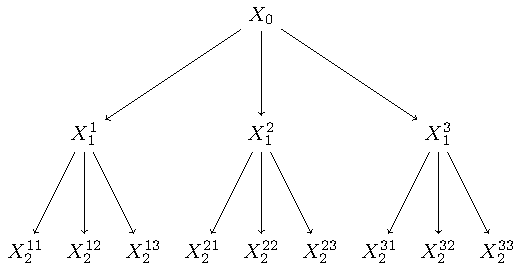
\includegraphics[width=\textwidth]{exponential_tree}
    \caption{Дерево состояний актива для $b = 3, m = 2$.}
    \label{fig:exponential_tree}
    \end{figure}
\end{frame}

\begin{frame}
    \frametitle{Постановка задачи} 
    Число вершин в дереве:
    $$\sum_{k=0}^m b^k = \frac{b^{m+1} - 1}{b-1} = O(b^m), \text{ при этом } m\to\infty.$$
    \bluetext{Задача:} указать методы, позволяющие избежать экспоненциального роста вычислительной работы. 
    \vskip 0.05\paperheight
    Избежать экспоненциального роста позволяет рандомизация.
\end{frame}

\begin{frame}
    \frametitle{Интегральные уравнения с полиномиальной нелинейностью} 
    В <<Методах Монте-Карло и смежных вопросах>> С.~М.~Ермакова для
    $$\vfi\left(x\right) = \int K\left(x, y_1, \ldots, y_b \right)\prod_{i=1}^b\vfi\left(y_i\right) \mu^b\left(dy_1\cdots dy_b\right) + f\left(x\right),$$
    описано использование случайных поддеревьев полного дерева
    \begin{figure}
    \centering
    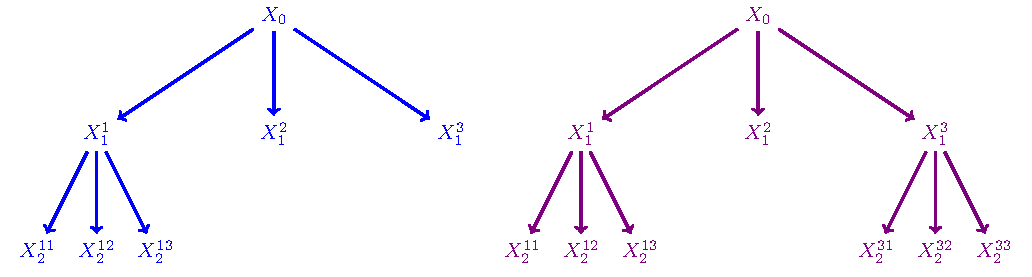
\includegraphics[width=\textwidth]{exponential_subtrees}
    \end{figure}
\end{frame}

\begin{frame}
    \frametitle{Интегральные уравнения с полиномиальной нелинейностью} 
    Также имеется сходство между самими уравнениями:
    \begin{align*}
        \vfi\left(x\right) = f\left(x\right) + &\int K\left(x, y_1, \ldots, y_b \right)\prod_{i=1}^b\vfi\left(y_i\right) \mu^b\left(dy_1\cdots dy_b\right) \text{ и } \\
        V_i(X_i) = h\left(X_i\right)\oplus &\int V_{i+1}p_{i, i+1}\left(X_i, X_{i+1}\right) dX_{i+1}.
    \end{align*}
    Можно проводить аналогии в построении оценок.
\end{frame}

\begin{frame}
    \frametitle{Механизм моделирования} 
    Заданы $p(X_k; X_{k+1}^1, \cdots, X_{k+1}^b)$ и $g_k(X_k)$, $X_0$.
    % \newline\newline
    % В каждом новом состоянии моделируется событие обрыва траектории. Если траектория не обрывается,
    % \newline\newline
    % то моделируем $b$ дочерних вершин с плотностью $\nicefrac{p(x_k; x_{k+1}^1, \cdots, x_{k+1}^b)}{1 - g_k(X_k)}$ и повторяем процесс в каждой из них,
    % \newline\newline
    % иначе возвращаемся к родительской вершине.
    \begin{algorithm*}[H]
      \SetKwProg{Fn}{def}{\string:}{}
      \SetKwInOut{Input}{input}\SetKwInOut{Output}{output}
      \SetKwFunction{generate}{generate}
      \SetKwFunction{Get}{Get}
      \Fn{\generate{$X_i, b$}}{
          \Input{текущее состояние $X_i^{j_1\cdots j_i}$ (включает в себя время $t_i$), число веток $b$}
          \BlankLine
          \Get{событие обрыва $\eta$ с вероятностью $g_k$}\;
          \If{$\eta$ произошло}{
                возвращаемся к родительской вершине\;
              }
          \emph{промоделировать состояния $\left\lbrace X_{i+1}^1\cdots X_{i+1}^1 \right\rbrace$}\;
          \For{$x \in \left\lbrace X_{i+1}^l \right\rbrace_{l=1}^k$}{
            \generate{$x, b$}\;
          }
        }
      % \caption{алгоритм моделирования дерева}\label{alg:random_subtree}
    \end{algorithm*}
\end{frame}

% \section{Случайные деревья}
%     \begin{frame}
%         \frametitle{Случайные траектории}
%         Будем оценивать $V_0(S_0)$ методом Монте-Карло.
%         Промоделируем много вариантов жизни базового актива. Траектория --- набор состояний $S_{t_1}, \ldots, S_{t_n}$.
%         \begin{figure}[h]
%             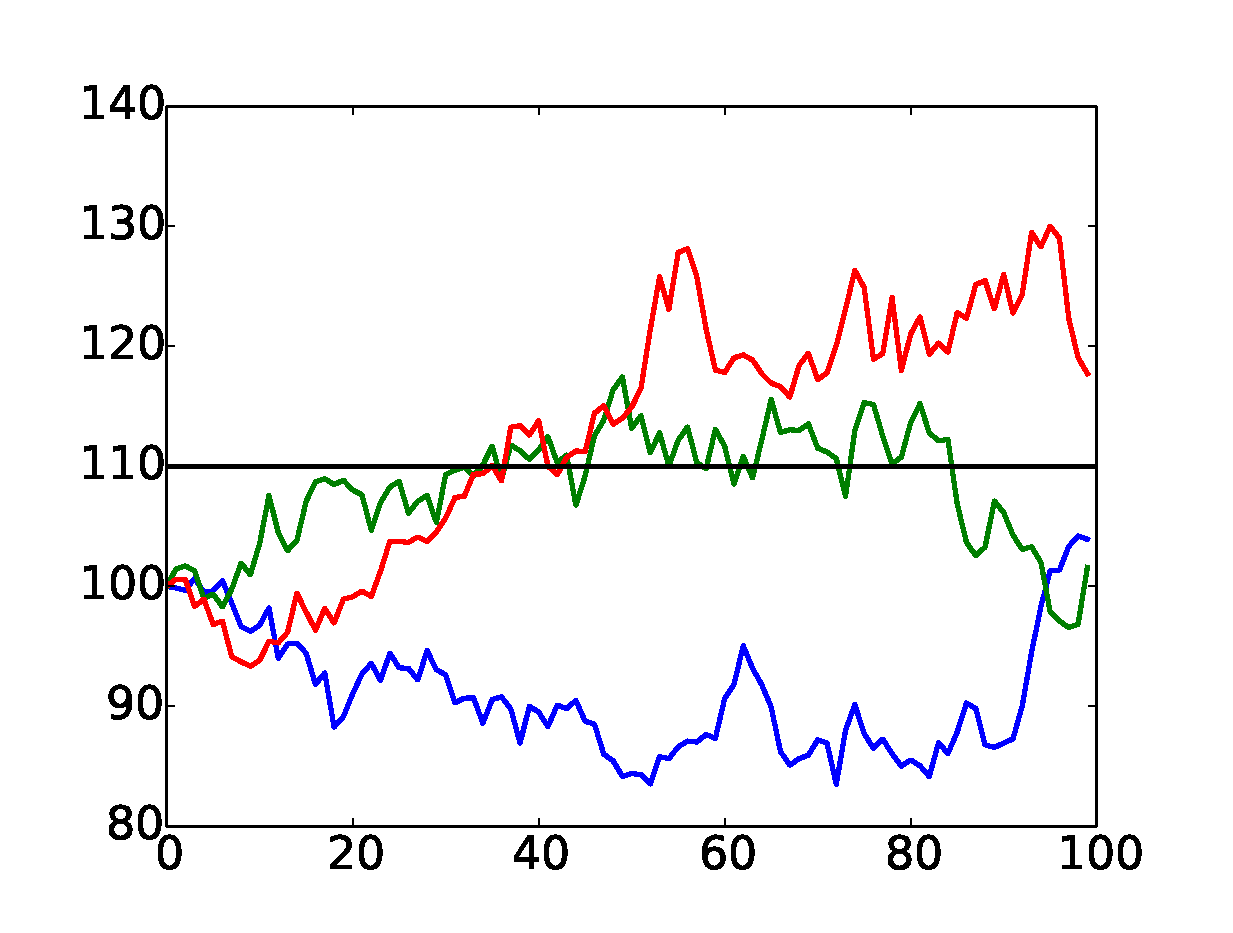
\includegraphics[height=0.5\paperheight]{traces}
%             \caption{Возможные траектории цены базового актива, горизонтальная линия --- цена страйк.}
%             \label{fig:traces}
%         \end{figure}
%     \end{frame}

% \begin{frame}
%     \frametitle{Случайные деревья}
%     Дерево --- способ получить больше траекторий в том же объёме памяти. Построение обычного дерева:
%     \begin{figure}
%     \centering
%     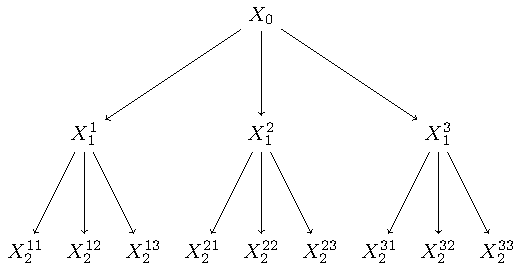
\includegraphics[width=\textwidth]{exponential_tree}
%     \caption{Дерево состояний актива для $b = 3, m = 2$.}
%     \label{fig:exponential_tree}
%     \end{figure}
% \end{frame}

% \begin{frame}
%     \frametitle{Случайные деревья}
%     Число вершин в дереве: $$\sum_{k=0}^n b^k = \frac{b^{n+1} - 1}{b-1} = O(b^n).$$
%     Схема Неймана-Улама для ветвящихся процессов даёт возможность обходить не все поддеревья.
%     \begin{figure}
%     \centering
%     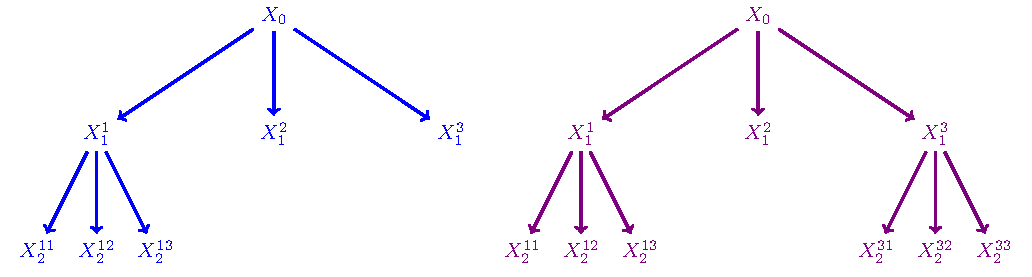
\includegraphics[width=\textwidth]{exponential_subtrees}
%     \end{figure}
% \end{frame}

% \begin{frame}
%     \frametitle{Оценка по поглощениям}
%     Для уравнений вида $$\vfi\left(x\right) = \int K\left(x, y, \vfi\left(y\right)\right)\vfi\left(y\right) \mu\left(dy\right) + f\left(x\right) \quad \mod \mu,$$
%     для которых сходится метод последовательных приближений 
%     \[
%     \vfi_n\left(x\right) = \int K\left(x, y, \vfi_{n-1}\left(y\right)\right)\vfi_n\left(y\right) \mu\left(dy\right) + f\left(x\right) \quad \mod \mu,
%     \]
%     разработан метод оценки по ветвящемуся марковскому процессу. Так как
%     $$
%     V_k\left(x\right) = h_k\left(x\right)\oplus \int V_{k+1}p_{k, k+1}\left(x, X_{k+1}\right) dX_{k+1},
%     $$
%     можно попробовать применить его к задаче оценки А.о.
% \end{frame}

% \begin{frame}
%     \frametitle{Оценка по поглощениям}
%     Доказано, что для оператора
%     \[
%     \begin{aligned}
%     A\left(\gamma\right) = &f\left[\nu(0)\right] \text{ при } N=0, \\
%     A\left(\gamma\right) = &a_{\nu(0)}\prod_{\GothB_1\setminus\GothB'_1}f\left[\nu(1)\right]\prod_{\GothB'_1}a_{\nu(1)} \prod_{\GothB_2\setminus\GothB'_2}f\left[\nu(1)\right]\prod_{\GothB'_2}a_{\nu(2)} \times \\
%     &\times\cdots\times \prod_{\GothB_N}f\left[\nu(N)\right] \text{ при } N>0,
%     \end{aligned}
%     \]
%     где $a_{\nu\left(k\right)}\vfi = \int K\left(
%             x\left[\nu(k)\right], x\left[\nu(k),1\right], \ldots ,x\left[\nu(k),b\right]
%         \right) \vfi d\mu$, 
%     \begin{block}{}
%     $$z\left[\nu(0)\right] = \sum_{\gamma\in\Gamma_N}A\left(\gamma\right)$$
%     \end{block}
% \end{frame}
% %     Доказано, что для оператора
% %     \[
% %     \begin{aligned}
% %     A\left(\gamma\right) = &f\left[\nu(0)\right] \text{ при } N=0, \\
% %     A\left(\gamma\right) = &a_{\nu(0)}\prod_{\GothB_1\setminus\GothB'_1}f\left[\nu(1)\right]\prod_{\GothB'_1}a_{\nu(1)} \prod_{\GothB_2\setminus\GothB'_2}f\left[\nu(1)\right]\prod_{\GothB'_2}a_{\nu(2)} \times \\
% %     &\times\cdots\times \prod_{\GothB_N}f\left[\nu(N)\right] \text{ при } N>0,
% %     \end{aligned}
% %     \]
% %     где $a_{\nu\left(k\right)}\vfi = \int K\left(
% %             x\left[\nu(k)\right], x\left[\nu(k),1\right], \ldots ,x\left[\nu(k),b\right]
% %         \right) \vfi d\mu$, 
% %     \begin{block}{}
% %     $$z\left[\nu(0)\right] = \sum_{\gamma\in\Gamma_N}A\left(\gamma\right)$$
% %     \end{block}
% % \end{frame}

\begin{frame}
    \frametitle{Результаты}
    \begin{columns}
        \begin{column}{0.5\textwidth}
            \begin{figure}[h]
                \centering
                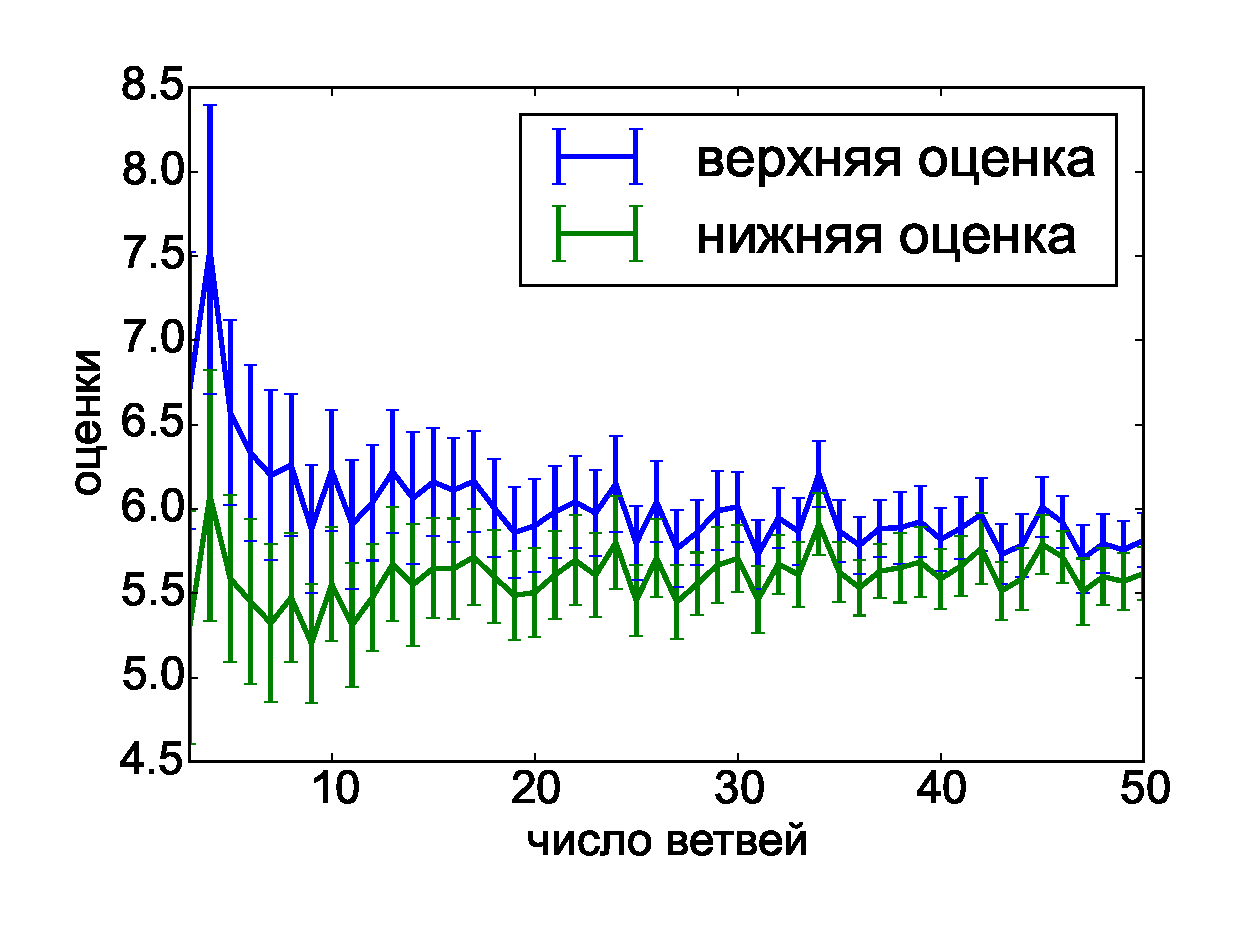
\includegraphics[width=\linewidth]{convergence_to_true_value_standard_slides}
                \caption{Полное дерево.}
                \label{fig:true_value_test_standard}
                \footnotesize{Реализация алгоритма из статьи}
            \end{figure}
        \end{column}
        \begin{column}{0.5\textwidth}
            \begin{figure}[h]
                \centering
                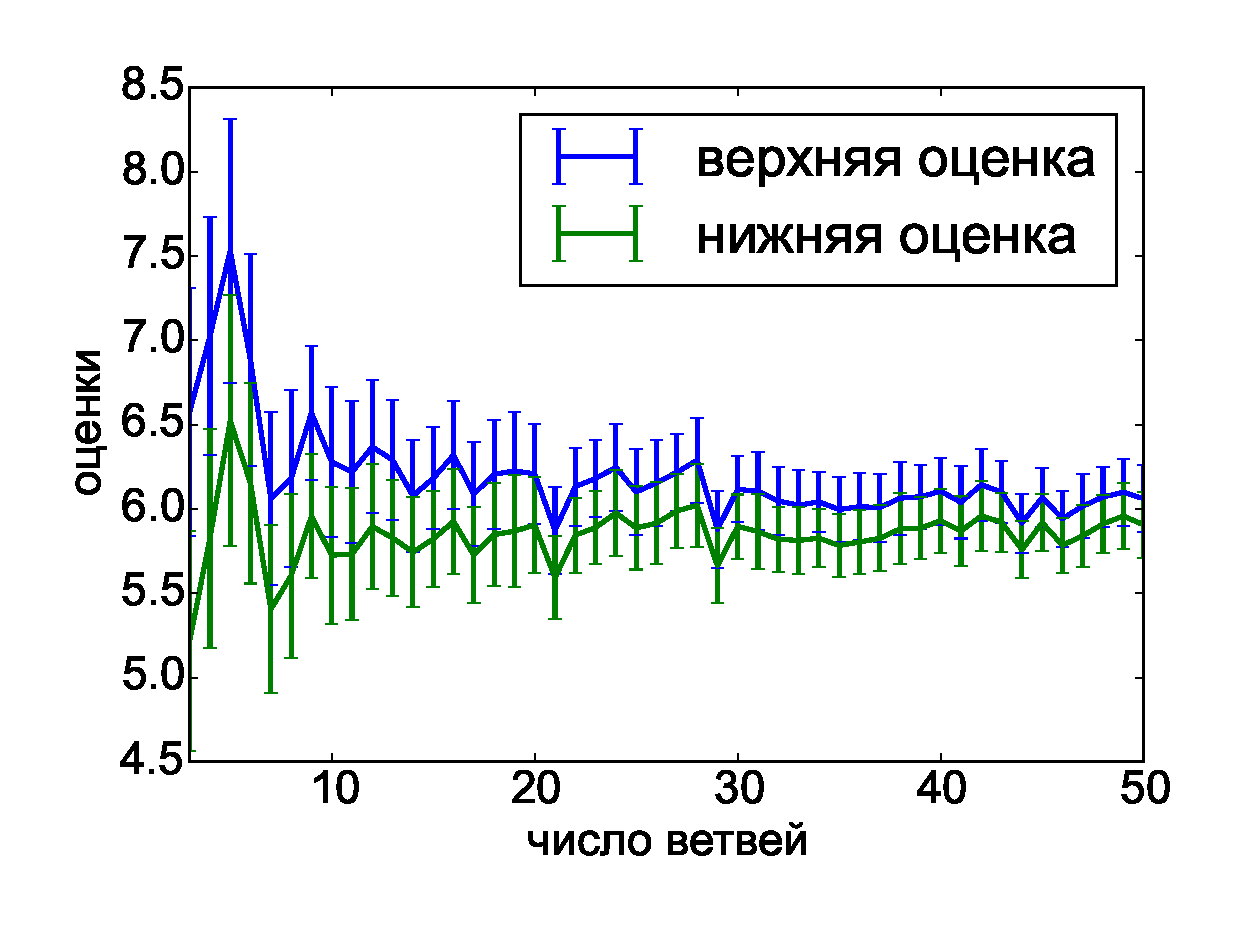
\includegraphics[width=\linewidth]{convergence_to_true_value_random_subtree_slides}
                \caption{Случайные поддеревья.}
                \label{fig:random_subtree_modified_ev}
                \footnotesize{Реализация предложенного в ВКР алгоритма}
            \end{figure}
        \end{column}
        
    \end{columns}
\end{frame}

\begin{frame}
    \frametitle{Результаты}
    \begin{columns}
        \begin{column}{0.5\textwidth}
            \begin{figure}[h]
                \centering
                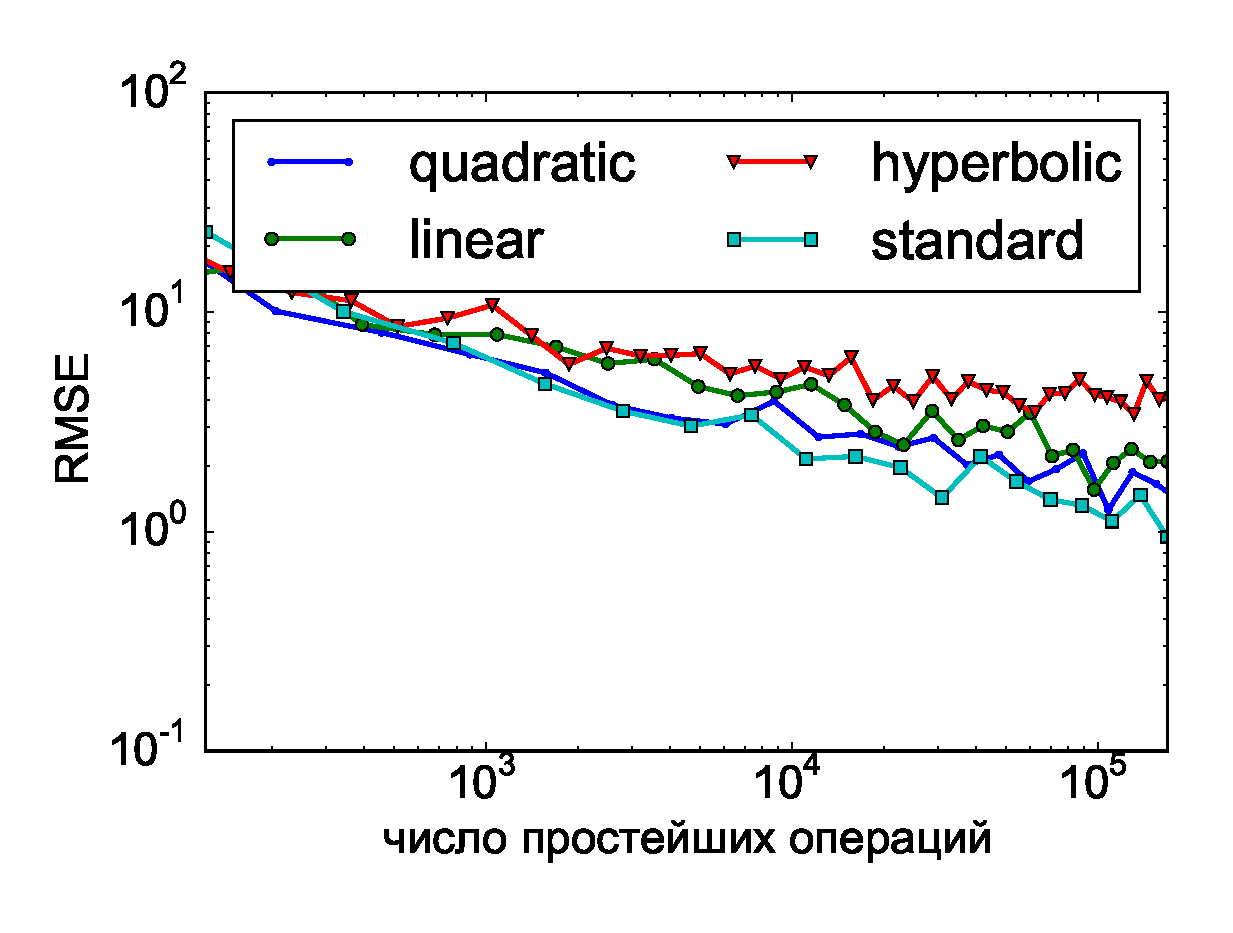
\includegraphics[width=\linewidth]{rmse_over_nop_upper_slides}
                \caption{Средняя ошибка оценки сверху}
                \label{fig:rmse_over_nop_standard_slides}
                % \footnotesize{Оценки стоимости опциона с начальной ценой 100, выписанного на срок 1 год на базовый актив с риск-нейтральной процентной ставкой $r = 0.05$, дивидендной ставкой $\delta = 0.1$ и волатильностью $\sigma=0.2$, цена которого --- случайный процесс, являющийся геометрическим броуновским движением с параметрами $\mu = r - \delta$ и $\sigma$, исполняемого 4 раза в году}
            \end{figure}
        \end{column}
        \begin{column}{0.5\textwidth}
            \begin{figure}[h]
                \centering
                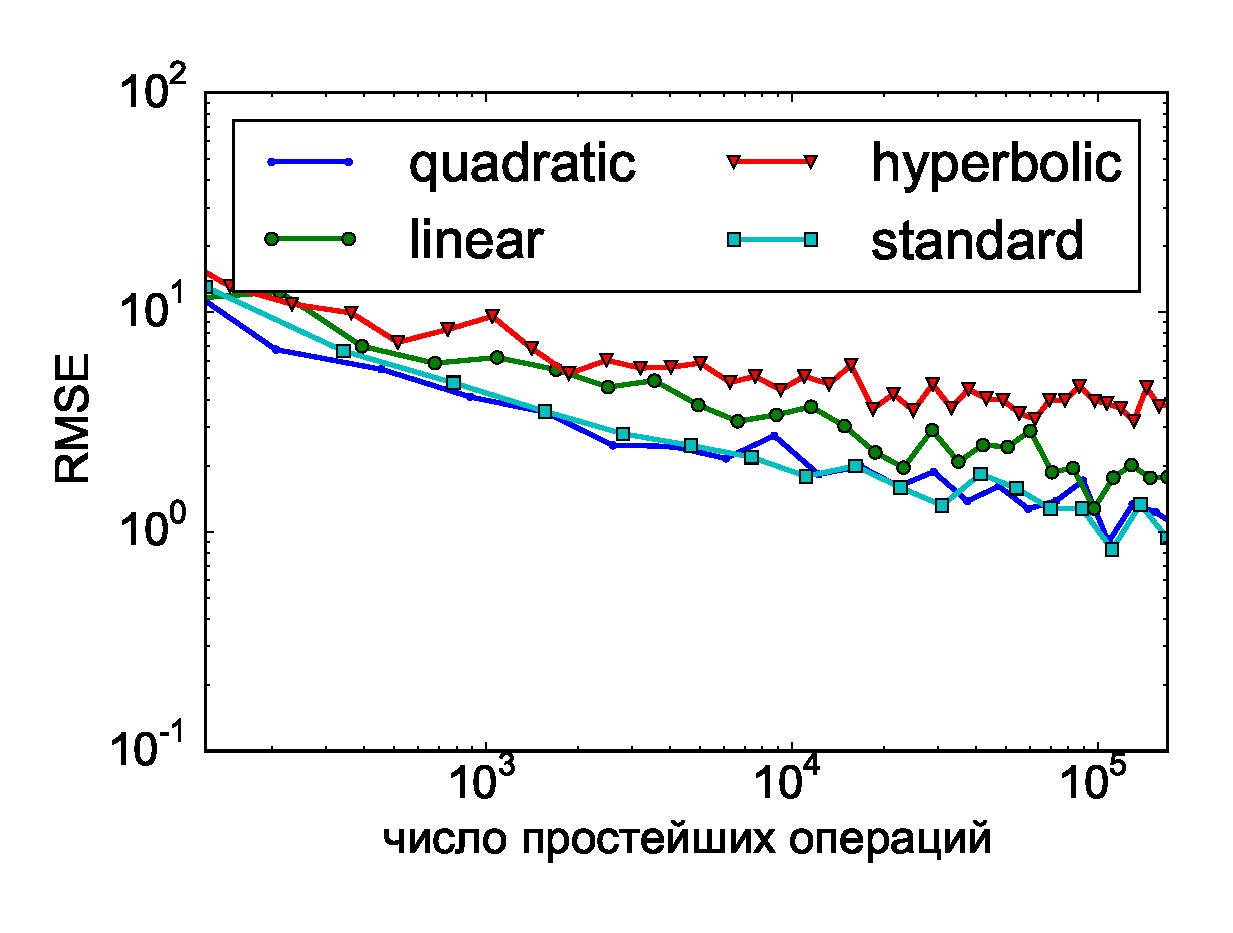
\includegraphics[width=\linewidth]{rmse_over_nop_lower_slides}
                \caption{Средняя ошибка оценки снизу}
                \label{fig:rmse_over_nop_random_subtree_slides}
                % \footnotesize{Оценки стоимости опциона с начальной ценой 100, выписанного на срок 1 год на базовый актив с риск-нейтральной процентной ставкой $r = 0.05$, дивидендной ставкой $\delta = 0.1$ и волатильностью $\sigma=0.2$, цена которого --- случайный процесс, являющийся геометрическим броуновским движением с параметрами $\mu = r - \delta$ и $\sigma$, исполняемого 4 раза в году}
            \end{figure}
        \end{column}
        
    \end{columns}
\end{frame}

\begin{frame}
    \frametitle{Итоги}
    \begin{itemize}
        \item Рассмотрены оценки Американских опционов, основанные на имитационных моделях.
        \item Проведены аналогии с решением интегральных уравнений с полиномиальной нелинейностью.
        \item Реализованы методы и проведены вычислительные эксперименты по подбору оптимального соотношения дисперсии и вычислительной сложности.
        \item Предложенный метод применим при больших $m$, когда исходный метод работает неприемлемо долго.
    \end{itemize}
\end{frame}

\end{document}
